\subsection{Deep-Taylor-Decomposition}\label{subsect:dtd}
\gls{dtd} as proposed by \fcite{Montavon.2017} tries to overcome the difficulties that the search for root-points according to \cref{enum:taylor-closeness} posed to simple \gls{td}. For this, they introduce axioms \ref{ax:positivity} and \ref{ax:consistency} which \gls{dtd} must satisfy. Also, they propose a method for finding root-points \(x_0(i):= x_i + t*v_i\), where \(v_i\) is called \textit{search direction}. \citeauthor{Montavon.2017} use this definition to define a set of weighting terms, similar to those in \gls{lrp} and \gls{td}. Formally, they introduce a generalization of the weighting parameter in \cref{eq:weighting-in-dtd}\cite[see][Supplementary Material]{Montavon.2017}
\begin{equation}
    R_{i\leftarrow j}^{(l,l+1)} = \sum_j \frac{v_i w_{ij}}{\sum_i v_i w_{ij}} R_j^{(l+1)}\label{eq:weighting-in-dtd}
\end{equation}
and then derive specific weighting parameters by defining \(v_i\).
\begin{description}
    \item[\namedlabel{itm:w2weighting}{\(\symbfit{w^2}\)-Weighting}{\(\symbfit{w^2}\)-weighting}] which is similar to \cref{eq:weighted-message} but does only rely on the weights \(w_{ij}\) that connect \(i \text{ and } j\). \(v_i\) is chosen to be \(v_i:=w_{ij}\).
    \begin{equation}
        R_{i\leftarrow j}^{(l,l+1)} = R_{j}^{(l+1)} \frac{w_{ij}^2}{\sum_{h\in (l)} w_{hj}^2}.\label{eq:w2-weighting-dtd}
    \end{equation}
    \(w^2\)-weighting is used, when the input-domain is unrestricted, i.e.\ \(x\in \mathbb R^{|x|}\).
    \item[\namedlabel{itm:z+weighting}{\(\symbfit{z^+}\)-Weighting}{\(\symbfit{z^+}\)-weighting}] is equal to the \(\alpha\beta\)-Rule of \gls{lrp}, with \(\beta=0, \alpha=1\). Here, \(v_i\) is the set of all \(x_i\) for which the correspoding \(w_{ij}\) is positive, formally \(w_{ij}^{+} = \left\{w_{ij} | w_{ij}\geq 0\right\}\) and \(v_i:=\left\{x_i|w_{ij}\in w_{ij}^{+}\right\}\). The weighting therefore is
    \begin{equation}
        R_{i\leftarrow j}^{(l,l+1)} = R_{j}^{(l+1)} \frac{x_i w_{ij}^{+}}{\sum_{h\in (l)} x_(h) w_{hj}^{+}}.\label{eq:dtd-z+}
    \end{equation}
    In~\cite{Montavon.2017}, \cref{eq:dtd-z+} is modeled with \(x_i w_{ij}^{+}=:z_{ij}^{+}\), from which the name \(z^{+}\)-weighting is derived.
    \(z^{+}\)-weighting is used, when the input-domain is restricted to positive values, for example in a setting with ReLU-activations, i.e.\ \(x\in \mathbb R_{+}^{|x|}\). A generalization of the \(z^{+}\)-weighting, as discussed in~\cite{Montavon.2017}, is equal to \(\alpha\beta\)-\gls{lrp}.
    \item[\(\symbfit{z^{\mathscr B}}\)-Weighting] is used, when the input-domain is restricted to an upper- and lower-bound, for example in image-classification tasks. For details, please refer to~\cite[215\psq]{Montavon.2017}
\end{description}
\par
In contrast to \gls{td}, \gls{dtd} defines not immediately the relevance at the input-sample \(R_{h}^{(1)}\), but only the relevance of \glspl{message}. It therefore incorporates ideas of both \gls{lrp} (relevance-propagation, even partial equality with the generalization of \ref{itm:z+weighting}) and \gls{td} (approximation of function value with respect to a root-point \(x_0\)). The relevance at the input-sample is recieved by a relevance model that then propagates the \glspl{message} from \(f(x)\) to \(R_{h}^{(1)}\).
\paragraph{Relevance-Models}
\begin{figure*}[ht]
    \center{}
    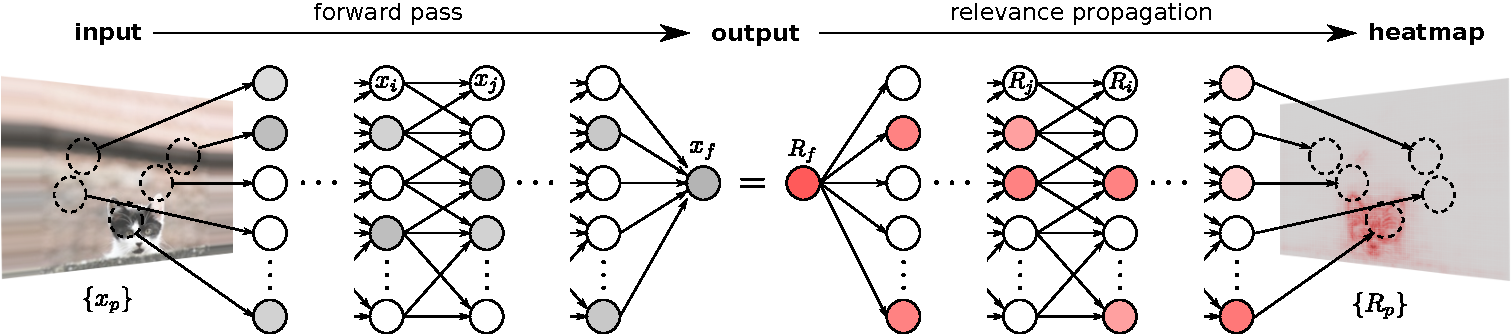
\includegraphics[width=\textwidth]{dtd-flow}
    \caption[Deeper Neural Network; prediction and propagation via \gls{dtd}]{\textbf{Left:} A neural network at prediction time. \textbf{Right:} exemplary \gls{dtd} Relevance Model, adopted from \protect\cite{Montavon.2017}. Note, that in this work, usually \(R_h\) is used instead of \(R_p\).}\label{fig:dtd-nn}
\end{figure*}
\fcite{Montavon.2017} propose two relevance models (\textit{Min-Max Relevance Model} and \textit{Training-free Relevance Model}), for which details are provided in~\cite{Montavon.2017}. They are presented as an inversion of the original \gls{nn}, incorporating their structure. However, no explicit constraints on this property are formulated. The flow in a relevance model is visually depicted in \cref{fig:dtd-nn}. First a prediction \(f(x)=:x_f\) is made (left side) which is then fed through the Relevance Model which extends \(R_f:=x_f\) back to the input sample. While the \textit{Training-free Relevance Model} must, as its name suggests, not be trained, the \textit{Min-Max Relevance Model} has to be trained in a supervised fashion. \fcite{Montavon.2017} show that both, the training-free and min-max relevance models, lead to very similar results.